\documentclass{article}
\usepackage{amsmath}
\usepackage{graphicx}
\usepackage{multicol}
\usepackage[margin=0.65in]{geometry}

\begin{document}
\section*{APPM 1350 Recitation, Fall 2021, Week 3, Sep 07}
\vspace{0.5in}

\subsection*{Limits with Graphs}
The graph of the function f is:\\
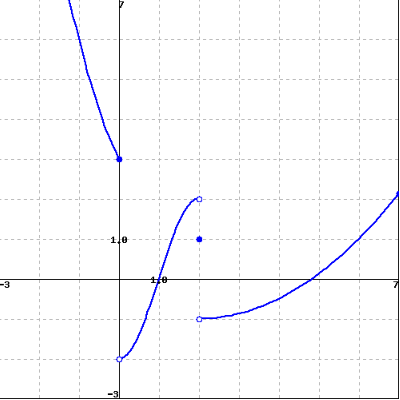
\includegraphics[scale=0.4]{func}

Evaluate the following:
\setlength{\columnsep}{-2.1in}
\begin{multicols}{2}
	\begin{itemize}
		\item $\lim_{x \rightarrow 0^-} f(x)$
		\item $\lim_{x \rightarrow 2} f(x)$
		\item $f(0)$
		\item $\lim_{x \rightarrow 0^+} f(x)$
		\item $\lim_{x \rightarrow 2^-} f(x)$
		\item $\lim_{x \rightarrow 2^+} f(x)$
		\item $f(2)$
		\item $\lim_{x\to 1} f(x)$
	\end{itemize}
\end{multicols}

\vspace{2cm}
\subsection*{Limits with Piecewise Functions}
\begin{align*}
f(x) = \begin{cases} 
-2x-5 & \text{if } x<-2 \\
x^2+1 & \text{if } -2 \leq x < 1 \\
2 & \text{if } x \geq 1 
\end{cases}
\end{align*}
Evaluate the following. At what values is the function discontinuous? 

\noindent
Use the definition of continuity to justify your answer.
\setlength{\columnsep}{-2.1in}
\begin{multicols}{2}
	\begin{itemize}
		\item $\lim_{x \rightarrow -2^-} f(x)$
		\item $\lim_{x \rightarrow -2^+} f(x)$
		\item $f(-2)$
		\item $f(1)$
		\item $\lim_{x \rightarrow 1^+} f(x)$
		\item $\lim_{x \rightarrow 1^-} f(x)$
	\end{itemize}
\end{multicols}

\pagebreak

\subsection*{Limits with Functions}
\begin{enumerate}
	\item Evaluate $\displaystyle \lim_{t \to 0} \frac{\sqrt{t^2+16} - 4}{t^2}$
	\item Evaluate $\displaystyle \lim_{x \to c} \frac{(x-2)|x-1|}{x^2 -3x +2}$ for $c=1^+, 1^-, 2^+, 2^-$
	\item Evaluate $\displaystyle \lim_{x \to 0}\frac{\sin{3x}}{5x}$
	\item Evaluate $\displaystyle \lim_{x \to 0} x^2 \cos\left(\frac{1}{x^2}\right)$
	\item Evaluate $\displaystyle \lim_{x \to 0} \frac{\sin{4x}}{5x^3-2x}.$ At what values is the function discontinuous?
	\item Evaluate $\displaystyle \lim_{h \to 0}\frac{(6+h)^2-36}{h}$
\end{enumerate}

\vspace{2cm}

\subsection*{Intermediate Value Theorem}

Use the Intermediate Value Theorem to show that the following equations have at least one solution:
\begin{enumerate}
	\item $x^{5}-6x^{3}+3x+1 = 0$
	\item $2\sin(x) = 3 - 2x $	
\end{enumerate}


\end{document}
